\documentclass[11pt,a4paper]{article}

% ---- Packages ----------------------------------------------------------
\usepackage[utf8]{inputenc}
\usepackage[T1]{fontenc}
\usepackage{lmodern}
\usepackage[margin=0.85in]{geometry}
\usepackage{microtype}
\usepackage{amsmath}
\usepackage{amssymb}
\usepackage{titlesec}
\usepackage{enumitem}
\usepackage{booktabs}
\usepackage{array}
\usepackage{tabularx}
\usepackage{xcolor}
\usepackage{graphicx}
\usepackage{fancyhdr}
\usepackage{tikz}
\usetikzlibrary{positioning, arrows.meta, shapes.geometric, fit, calc, backgrounds, decorations.pathreplacing}
\usepackage[hidelinks,colorlinks=true,linkcolor=black,citecolor=violet,urlcolor=violet]{hyperref}
\usepackage{parskip}
\usepackage{float}
\usepackage{tcolorbox}
\tcbuselibrary{skins, breakable}

% ---- Colours -----------------------------------------------------------
\definecolor{primary}{HTML}{4338CA}
\definecolor{primarylight}{HTML}{E0E7FF}
\definecolor{secondary}{HTML}{0E7490}
\definecolor{secondarylight}{HTML}{CFFAFE}
\definecolor{accent}{HTML}{C2410C}
\definecolor{accentlight}{HTML}{FFEDD5}
\definecolor{ink}{HTML}{1E1B4B}
\definecolor{mute}{HTML}{64748B}
\definecolor{mutelight}{HTML}{F1F5F9}
\definecolor{precfp}{HTML}{0F766E}      % fp16 colour (deep teal)
\definecolor{precfplight}{HTML}{CCFBF1}
\definecolor{precint}{HTML}{7C3AED}     % int8 colour (violet)
\definecolor{precintlight}{HTML}{EDE9FE}
\definecolor{clsA}{HTML}{0F766E}
\definecolor{clsAlight}{HTML}{CCFBF1}
\definecolor{clsB}{HTML}{B45309}
\definecolor{clsBlight}{HTML}{FEF3C7}
\definecolor{clsC}{HTML}{BE185D}
\definecolor{clsClight}{HTML}{FCE7F3}
\definecolor{clsN}{HTML}{4338CA}        % new class colour
\definecolor{clsNlight}{HTML}{E0E7FF}

% ---- TikZ styles -------------------------------------------------------
\tikzset{
  block/.style    = {rectangle, rounded corners=3pt, draw=primary, thick,
                     fill=primarylight, minimum width=2.6cm, minimum height=0.85cm,
                     align=center, font=\small},
  data/.style     = {rectangle, rounded corners=3pt, draw=mute, thick,
                     fill=mutelight, minimum width=2.4cm, minimum height=0.8cm,
                     align=center, font=\small},
  int8/.style     = {rectangle, rounded corners=3pt, draw=precint, thick,
                     fill=precintlight, minimum width=3.2cm, minimum height=0.7cm,
                     align=center, font=\small},
  fp16/.style     = {rectangle, rounded corners=3pt, draw=precfp, very thick,
                     fill=precfplight, minimum width=3.2cm, minimum height=1.3cm,
                     align=center, font=\small},
  decision/.style = {diamond, draw=accent, thick, fill=accentlight, aspect=1.6,
                     inner sep=1pt, align=center, font=\small},
  result/.style   = {rectangle, rounded corners=3pt, draw=accent, thick,
                     fill=accentlight, minimum width=2.4cm, minimum height=0.8cm,
                     align=center, font=\small},
  ar/.style       = {-{Latex[length=2mm,width=1.6mm]}, thick, draw=ink!75},
}

% ---- Header / Footer ---------------------------------------------------
\pagestyle{fancy}
\fancyhf{}
\fancyhead[L]{\small\color{primary}\textbf{Quantisation \& Continual Learning}}
\fancyhead[R]{\small\color{mute}Madhav Dogra}
\fancyfoot[C]{\small\color{mute}\thepage}
\renewcommand{\headrulewidth}{0pt}

% ---- Section format ----------------------------------------------------
\titleformat{\section}
  {\normalfont\LARGE\bfseries\color{primary}}
  {\textcolor{accent}{\thesection}\hspace{0.4em}}{0pt}{}
\titlespacing*{\section}{0pt}{14pt}{6pt}

\titleformat{\subsection}
  {\normalfont\large\bfseries\color{ink}}
  {\textcolor{secondary}{\thesubsection}\hspace{0.3em}}{0pt}{}
\titlespacing*{\subsection}{0pt}{8pt}{2pt}

\setlength{\parskip}{4pt}

\tcbset{
  idea/.style={colback=secondarylight, colframe=secondary!60, boxrule=0.5pt,
               arc=2pt, left=8pt, right=8pt, top=5pt, bottom=5pt,
               fonttitle=\bfseries\small, coltitle=white, colbacktitle=secondary,
               title={\strut KEY POINT}},
}

% =======================================================================
\begin{document}

\begin{center}
{\color{primary}\rule{\linewidth}{1pt}}\\[6pt]
{\Huge\bfseries\color{ink} Quantisation \& Continual Learning} \\[6pt]
{\Large\color{secondary} Deployment notes for the Mamba IoT anomaly detector} \\[4pt]
{\color{mute}\rule{0.6\linewidth}{0.3pt}}\\[4pt]
{\normalsize\color{mute} Madhav Dogra}
\end{center}

\vspace{4pt}

% =======================================================================
\section{Quantising the Mamba detector}

The deployed detector has to fit on gateway-class hardware --- Raspberry-Pi-class, single-digit watts. Quantisation, storing weights and activations in fewer bits than the default fp32, is the standard route to a smaller, faster model. The question is whether Mamba quantises cleanly, since most published quantisation work targets transformers.

\begin{tcolorbox}[idea]
Mamba does quantise, but the selective state-space core has activation outliers that compound through its recurrence. The practical strategy is \emph{mixed precision}: int8 for the linear projections (most of the parameters), fp16 for the SSM core (the sensitive part). Three benchmark rows --- fp32, int8 everywhere, mixed precision --- let the operator pick.
\end{tcolorbox}

\subsection{Why Mamba is harder than transformers to quantise}

A Mamba block has two parts. The \textbf{linear projections} (input, gating, output) dominate the parameter count and quantise cleanly to int8. The \textbf{selective state-space core} (discretisation via $\Delta$, the input-dependent $B$, $C$, and the recurrent scan) has activation outliers --- magnitude concentrated in a few channels --- and errors compound along the sequence through the recurrence. Int8 can't represent these without large quantisation error.

Headline recipe: \emph{int8 the projections, fp16 the SSM core.} Size savings come mostly from the projections anyway.

% ---- Figure 1: Mamba block precision split ----------------------------
\begin{figure}[H]
\centering
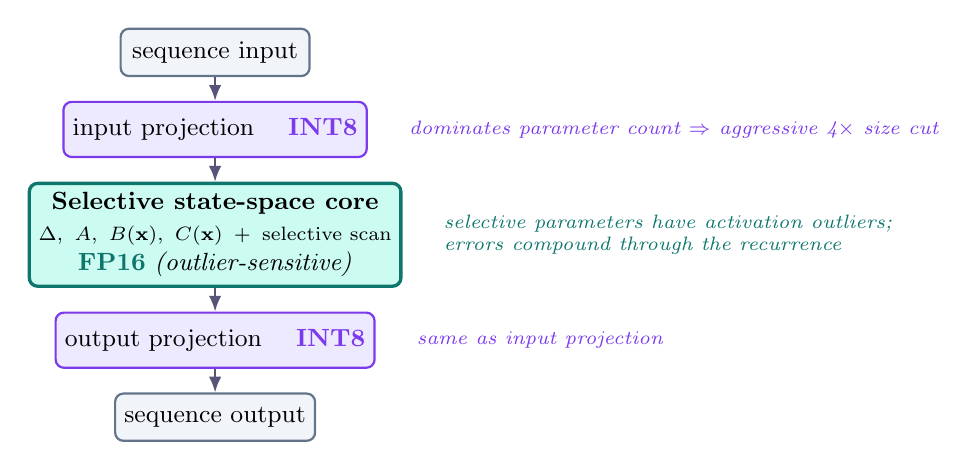
\begin{tikzpicture}[node distance=0.3cm and 0.6cm]

  \node[data, minimum width=2.4cm, minimum height=0.6cm] (in) {sequence input};
  \node[int8, below=of in] (proj1) {input projection \quad\textcolor{precint}{\textbf{INT8}}};
  \node[fp16, below=of proj1] (ssm)
       {\textbf{Selective state-space core} \\
        \scriptsize $\Delta,~A,~B(\mathbf{x}),~C(\mathbf{x})$ \,+\, selective scan \\
        \textcolor{precfp}{\textbf{FP16}} \emph{(outlier-sensitive)}};
  \node[int8, below=of ssm] (proj2) {output projection \quad\textcolor{precint}{\textbf{INT8}}};
  \node[data, below=of proj2, minimum width=2.4cm, minimum height=0.6cm] (out) {sequence output};

  \draw[ar] (in) -- (proj1);
  \draw[ar] (proj1) -- (ssm);
  \draw[ar] (ssm) -- (proj2);
  \draw[ar] (proj2) -- (out);

  \node[font=\scriptsize\itshape\color{precint}, align=left, right=0.4cm of proj1]
       {dominates parameter count $\Rightarrow$ aggressive 4$\times$ size cut};
  \node[font=\scriptsize\itshape\color{precfp}, align=left, right=0.4cm of ssm]
       {selective parameters have activation outliers;\\errors compound through the recurrence};
  \node[font=\scriptsize\itshape\color{precint}, align=left, right=0.4cm of proj2]
       {same as input projection};

\end{tikzpicture}
\caption*{\small\textit{Figure 1 --- Mixed-precision split inside a Mamba block. Linear projections (violet, int8) carry most of the weights and quantise cleanly. The selective SSM core (teal, fp16) is sensitive and stays at higher precision. This is the practical compromise across the 2024--25 Mamba quantisation literature (Q-Mamba, MambaQuant, PTQ4SSM).}}
\end{figure}

\subsection{Benchmark plan}
We will report the deployed model in three precisions, so the operator can choose:

\begin{center}
\small
\begin{tabularx}{\linewidth}{@{}Xccc@{}}
\toprule
\textbf{Configuration} & \textbf{Size} & \textbf{p95 latency} & \textbf{Accuracy hit} \\
\midrule
fp32 (baseline)                                 & $1.0\times$         & $1.0\times$         & --- \\
int8 PTQ everywhere                             & $0.25\times$        & ${\sim}0.5\times$   & risk on SSM core \\
\textbf{Mixed precision (recommended)}          & $\approx 0.30\times$ & ${\sim}0.55\times$ & smallest drop \\
\bottomrule
\end{tabularx}
\end{center}

If the int8-everywhere row degrades accuracy too far, the mixed-precision row is our recommended deployment configuration. \textbf{QAT (quantisation-aware training)} is a fallback for the SSM core if even fp16 leaves quality on the table at deployment.

% =======================================================================
\section{Class correlation in progressive learning}

The detector must absorb new attack types as they appear in the wild --- without retraining the encoder from scratch, and without forgetting the existing classes. The hard case is correlation: a new attack class often looks like an existing one (e.g., a new DDoS variant resembling the standard DDoS class), so naive head retraining will quietly confuse them.

\begin{tcolorbox}[idea]
A replay buffer of old-class examples handles most cases. Before committing a new class label, run an embedding-space check on a sample of the new attack flows --- merge with an existing class if they overlap, enforce separation via margin loss if they sit between classes. Uncertain predictions are surfaced to the SOC rather than forced into a hard label.
\end{tcolorbox}

\subsection{What goes wrong with naive head retraining}

Three failure modes appear when the new class correlates with an old one: \textbf{catastrophic forgetting} (head drifts toward the new class, misclassifies the old one), \textbf{probability-mass theft} (the new softmax dimension steals confidence from the correlated class even on examples the model used to get right), and \textbf{spurious hard labels} (boundary flows get forced into one class with high confidence, hiding the real ambiguity from the analyst).

\subsection{The embedding-space view --- three scenarios}

Before adding a new class, embed the candidate attack flows via the frozen encoder and inspect where they land in the existing embedding space. Three outcomes:

% ---- Figure 2: Embedding-space scenarios (compact, 3-up) ---------------
\begin{figure}[H]
\centering
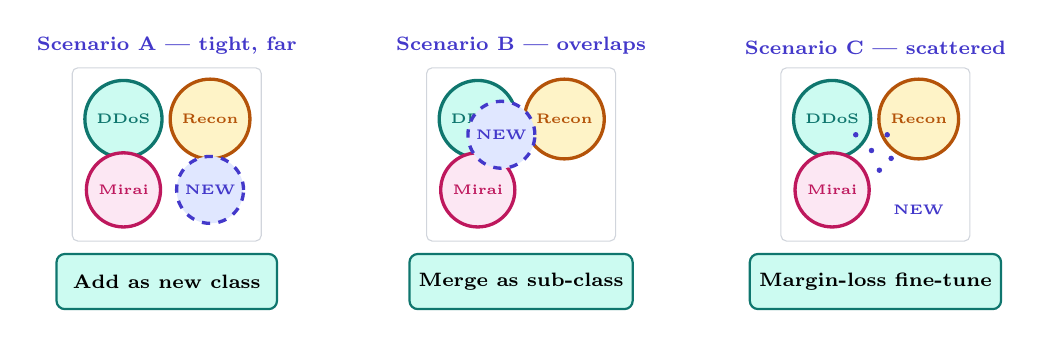
\begin{tikzpicture}[
    cluster/.style 2 args={circle, draw=#1, very thick, fill=#1!8, inner sep=0pt, minimum size=0.85cm, font=\tiny\color{#1}\bfseries, label=center:#2},
    clusterN/.style={circle, draw=clsN, dashed, very thick, fill=clsNlight, inner sep=0pt, minimum size=0.85cm, font=\tiny\color{clsN}\bfseries},
    dotN/.style={circle, fill=clsN, inner sep=0.7pt},
    scene/.style={draw=mute!30, rounded corners=2pt},
  ]

  % Scenario A
  \begin{scope}[local bounding box=A]
    \draw[scene] (-1.2,-1.1) rectangle (1.2,1.1);
    \node[circle, draw=clsA, very thick, fill=clsAlight, minimum size=0.85cm, font=\tiny\color{clsA}\bfseries] at (-0.55, 0.45) {DDoS};
    \node[circle, draw=clsB, very thick, fill=clsBlight, minimum size=0.85cm, font=\tiny\color{clsB}\bfseries] at ( 0.55, 0.45) {Recon};
    \node[circle, draw=clsC, very thick, fill=clsClight, minimum size=0.85cm, font=\tiny\color{clsC}\bfseries] at (-0.55, -0.45) {Mirai};
    \node[clusterN] at (0.55, -0.45) {NEW};
  \end{scope}
  \node[font=\bfseries\scriptsize\color{primary}, above=0.05cm of A] {Scenario A --- tight, far};
  \node[result, below=0.15cm of A, minimum width=2.8cm, fill=clsAlight, draw=clsA, font=\scriptsize, minimum height=0.7cm]
       {\textbf{Add as new class}};

  % Scenario B
  \begin{scope}[local bounding box=B, shift={(4.5,0)}]
    \draw[scene] (-1.2,-1.1) rectangle (1.2,1.1);
    \node[circle, draw=clsA, very thick, fill=clsAlight, minimum size=0.85cm, font=\tiny\color{clsA}\bfseries] at (-0.55, 0.45) {DDoS};
    \node[circle, draw=clsB, very thick, fill=clsBlight, minimum size=0.85cm, font=\tiny\color{clsB}\bfseries] at ( 0.55, 0.45) {Recon};
    \node[circle, draw=clsC, very thick, fill=clsClight, minimum size=0.85cm, font=\tiny\color{clsC}\bfseries] at (-0.55, -0.45) {Mirai};
    \node[clusterN] at (-0.25, 0.25) {NEW};
  \end{scope}
  \node[font=\bfseries\scriptsize\color{primary}, above=0.05cm of B] {Scenario B --- overlaps};
  \node[result, below=0.15cm of B, minimum width=2.8cm, fill=clsAlight, draw=clsA, font=\scriptsize, minimum height=0.7cm]
       {\textbf{Merge as sub-class}};

  % Scenario C
  \begin{scope}[local bounding box=C, shift={(9.0,0)}]
    \draw[scene] (-1.2,-1.1) rectangle (1.2,1.1);
    \node[circle, draw=clsA, very thick, fill=clsAlight, minimum size=0.85cm, font=\tiny\color{clsA}\bfseries] at (-0.55, 0.45) {DDoS};
    \node[circle, draw=clsB, very thick, fill=clsBlight, minimum size=0.85cm, font=\tiny\color{clsB}\bfseries] at ( 0.55, 0.45) {Recon};
    \node[circle, draw=clsC, very thick, fill=clsClight, minimum size=0.85cm, font=\tiny\color{clsC}\bfseries] at (-0.55, -0.45) {Mirai};
    \node[dotN] at (-0.05, 0.05) {};
    \node[dotN] at ( 0.15, 0.25) {};
    \node[dotN] at (-0.25, 0.25) {};
    \node[dotN] at ( 0.2, -0.05) {};
    \node[dotN] at ( 0.05, -0.2) {};
    \node[font=\tiny\color{clsN}\bfseries] at (0.55, -0.7) {NEW};
  \end{scope}
  \node[font=\bfseries\scriptsize\color{primary}, above=0.05cm of C] {Scenario C --- scattered};
  \node[result, below=0.15cm of C, minimum width=2.8cm, fill=clsAlight, draw=clsA, font=\scriptsize, minimum height=0.7cm]
       {\textbf{Margin-loss fine-tune}};

\end{tikzpicture}
\caption*{\small\textit{Figure 2 --- Three embedding-space scenarios for a new attack class. Existing class clusters in solid colours; new class shown dashed (indigo). The geometric outcome dictates the strategy: tight \& far $\to$ add; overlapping $\to$ merge as sub-class; scattered between $\to$ enforce separation via margin loss. Run on a sample of the new flows \emph{before} any softmax change is committed.}}
\end{figure}

\subsection{The update protocol --- four defences, in order}

\begin{enumerate}[leftmargin=*, itemsep=3pt]
  \item \textbf{Replay buffer (primary).} Persist $\sim$100--500 labelled flows per existing class alongside the model. When fine-tuning the head on the new class, batch in replay examples so the head still sees every old class on every step. Cheap, well-studied, usually enough on its own.

  \item \textbf{Knowledge distillation (Learning-without-Forgetting).} During the fine-tune, regularise the new head toward agreeing with the old head's outputs on old-class data. Soft-target loss term added to the cross-entropy. Cost: one extra forward pass through the frozen old head.

  \item \textbf{Embedding-space sanity check.} Run the new attack samples through the frozen encoder, cluster the resulting embeddings, and locate them relative to existing class prototypes. Branch on the three scenarios in Figure~2.

  \item \textbf{Surface uncertainty, don't force labels.} If the softmax is split (e.g., 55\% NEW, 40\% DDoS), don't pick one. Pass both confidences plus the anomaly score and SHAP attributions to the SOC. The analyst gets the real picture instead of a confident wrong answer.
\end{enumerate}

% ---- Figure 3: Update protocol flowchart -------------------------------
\begin{figure}[H]
\centering
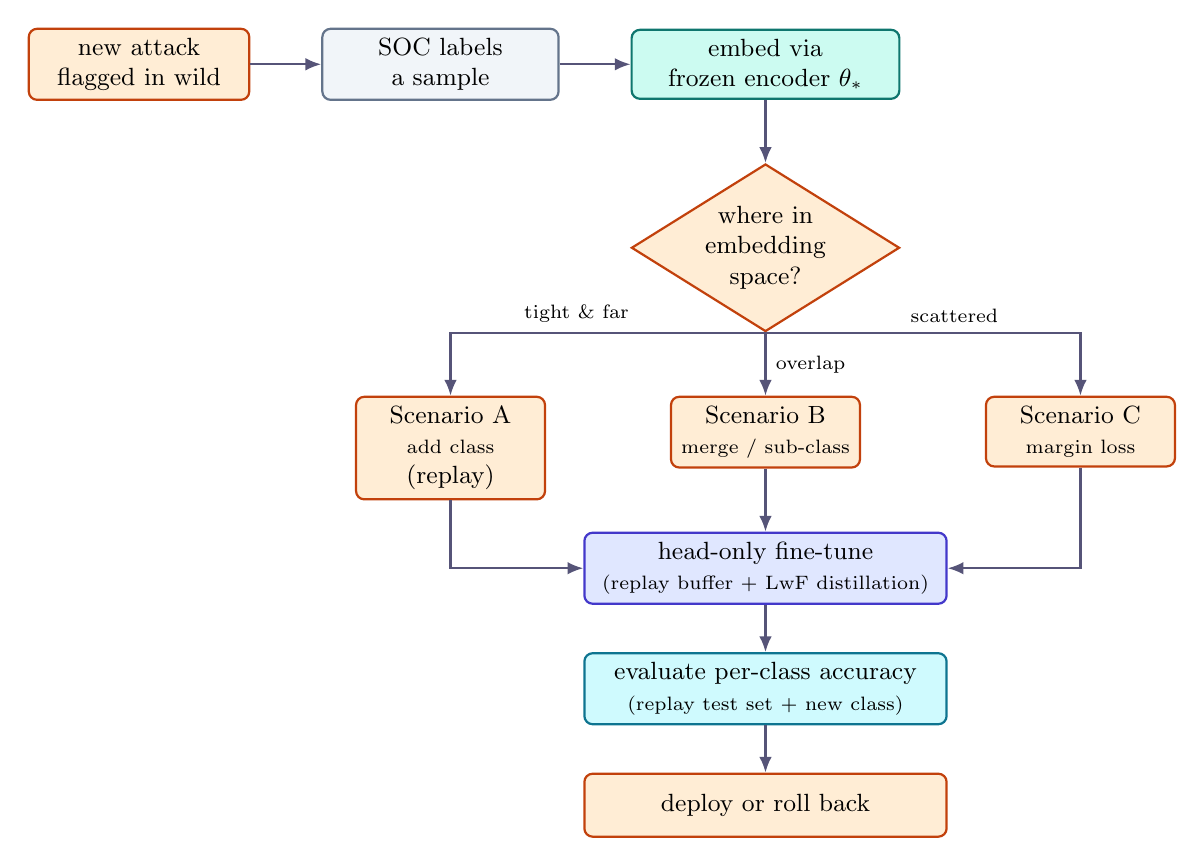
\begin{tikzpicture}[node distance=0.6cm and 0.9cm]

  \node[data, fill=accentlight, draw=accent, minimum width=2.8cm] (in) {new attack \\ flagged in wild};

  \node[block, right=of in, minimum width=3.0cm, fill=mutelight, draw=mute] (label)
       {SOC labels \\ a sample};

  \node[block, right=of label, minimum width=3.4cm, fill=precfplight, draw=precfp] (embed)
       {embed via \\ frozen encoder $\theta_*$};

  \draw[ar] (in) -- (label);
  \draw[ar] (label) -- (embed);

  \node[decision, below=0.8cm of embed, fill=accentlight, draw=accent] (where)
       {where in \\ embedding \\ space?};

  \draw[ar] (embed) -- (where);

  \node[result, below=0.8cm of where, xshift=-4.0cm] (sA)
       {Scenario A \\ \scriptsize add class \\ (replay)};
  \node[result, below=0.8cm of where] (sB)
       {Scenario B \\ \scriptsize merge / sub-class};
  \node[result, below=0.8cm of where, xshift=4.0cm] (sC)
       {Scenario C \\ \scriptsize margin loss};

  \draw[ar] (where.south) -| node[pos=0.3, above, font=\scriptsize] {tight \& far} (sA.north);
  \draw[ar] (where) -- node[right, font=\scriptsize] {overlap} (sB);
  \draw[ar] (where.south) -| node[pos=0.3, above, font=\scriptsize] {scattered} (sC.north);

  \node[block, below=0.8cm of sB, minimum width=4.6cm, fill=primarylight, draw=primary] (update)
       {head-only fine-tune \\ \scriptsize (replay buffer + LwF distillation)};

  \draw[ar] (sA.south) |- (update.west);
  \draw[ar] (sB) -- (update);
  \draw[ar] (sC.south) |- (update.east);

  \node[block, below=of update, minimum width=4.6cm, fill=secondarylight, draw=secondary] (eval)
       {evaluate per-class accuracy \\ \scriptsize (replay test set + new class)};
  \draw[ar] (update) -- (eval);

  \node[result, below=of eval, minimum width=4.6cm] (out)
       {deploy or roll back};
  \draw[ar] (eval) -- (out);

\end{tikzpicture}
\caption*{\small\textit{Figure 3 --- The progressive-learning update protocol. The encoder is never touched. The SOC labels a sample of the new attack; the embedding-space scenario determines whether to add, merge, or separate via margin loss; the head is fine-tuned with replay and distillation; per-class accuracy is checked against a held-out test set before deploying. If any existing class regresses, the update is rolled back and the protocol restarts.}}
\end{figure}

After every head update, the per-class confusion matrix on a fixed held-out test set is recomputed. If \emph{any} existing class's F1 drops below an agreed threshold (e.g., 2 percentage points), the update is automatically rolled back and the SOC is alerted --- catastrophic forgetting is detected immediately, not weeks later.

\end{document}
